\documentclass{article}
\usepackage[colorlinks=true]{hyperref}
\usepackage[usenames,dvipsnames]{xcolor}
\usepackage{titling}
\usepackage{listings}
\usepackage{enumitem,multicol}
\usepackage{lmodern}
\usepackage{tcolorbox}
\usepackage{tikz}
\newcommand*\circled[1]{\tikz[baseline=(char.base)]{%
			\node[shape=circle,fill=blue!20,draw,inner sep=2pt] (char) {#1};}}
\usepackage[letterpaper]{geometry}
\geometry{verbose,tmargin=0.75in,bmargin=0.75in,lmargin=0.75in,rmargin=0.75in}

\newcommand{\subtitle}[1]{%
  \posttitle{%
    \par\end{center}
    \begin{center}\large#1\end{center}
    \vskip0.5em}%
}

\lstset{%set Code listings styles
	language=Java, % program language for keywords and comments styles
	basicstyle=\small, %font size and style
	identifierstyle=\color{black}, %variable name style
	stringstyle=\ttfamily, %string style
	keywordstyle=\color{blue}\bfseries, %language keyword style
	commentstyle=\color{OliveGreen}\itshape, %commentstyle
	breaklines=true,  % sets automatic line breaking
	breakatwhitespace=false,   %break line not just at whitespaces
	showspaces=false,
	showstringspaces=false,
}

\title{``Rock-Paper-Scissors-Lizard-Spock''}
\subtitle{Java Programming Lab}
\author{Concepts of Programming Languages\\CSCI 305, Spring 2018}
\date{Due: 3/25/2015 @ 12:30 PM}

\begin{document}

\maketitle

\section*{Java}
For this lab you will use Java. Java is already install on all machines in teh lab, and is provided by the Virtual Machine for this course. On the off chance you wish to install Java yourself, please visit http://www.oracle.com/java

All students should use Java 8 Standard Edition for this lab.

\section*{Game Overview}
Rock-paper-scisors-lizard-Spock is a five-gesture expansion of the classic game rock-paper-scissors. The game was invented by Sam Kass, but popularized in the clip from the TV show ``Big Bang Theory'': \url{https://www.youtube.com/watch?v=x5Q6-wMx-K8}. You may also find the wikipedia page useful:

\begin{center} \url{http://en.wikipedia.org/wiki/Rock-paper-scissors-lizard-Spock.} \end{center}

\noindent This diagram explains the outcomes of the game:

\begin{center}
 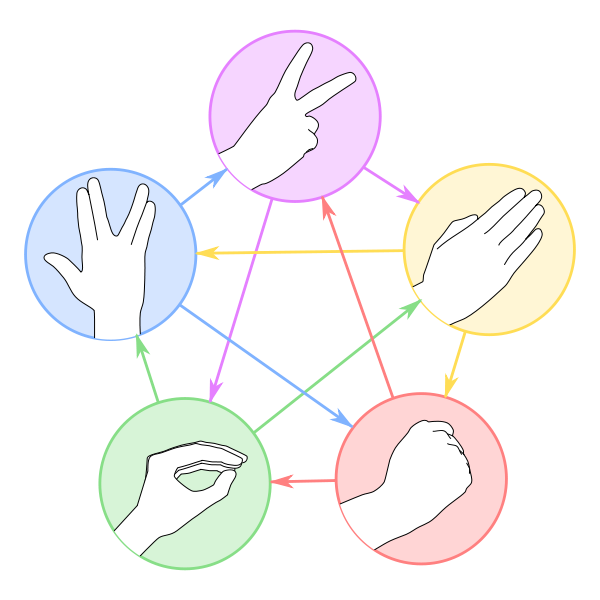
\includegraphics[scale=0.25]{images/RPSLS.png}
\end{center}


\section*{Implementation}
For this lab, you will implement this game, in Java, in an object-oriented way.
\\\\
\noindent Failure to implement the game using OO paradigms (as described below) will result in a significant loss of points.

\section*{Element Class}
First create a class named \verb|Element|. This class will serve as the superclass to five subclasses: \verb|Rock, Paper, Scissors,| \verb|Lizard, Spock|.
\\\\
\noindent The \verb|Element| class has one instance variable \verb|name|, which will sgtore the name of the Element (e.g., ``Rock'', ``Lizard'', etc). The constructor will take a name as a parameter and will save it to the instance variable \verb|name|. Next, create a getter method called \verb|getName()| that returns the instance variable \verb|name|. Lastely, create an abstract method \verb|compareTo| that takes an isntance of the class \verb|Element| as an argument. You will instantiate the method in the five concrete subclasses.
\\\\
\noindent As the next step, create your five subclasses: \verb|Rock, Paper, Scisssors, Lizard, Spock|. For each you should only need to implement (override) the \verb|compareTo| method. Since Java does not allow you to return multiple types, you will need a small class called \verb|Outcome|. \verb|Outcome| has two instance variables representing the outcome of the \verb|compareTo| method.
\\\\
\noindent The first value contained in the \verb|Outcome| class contains a string describing one of the following outcomes:
\begin{multicols}{2}
 \begin{itemize}
  \item Scissors cut Paper
  \item Paper covers Rock
  \item Rock crushes Lizard
  \item Lizard poisons Spock
  \item Spock smashes Scissors
  \item Scissors decapitate Lizard
  \item Lizard eats Paper
  \item Paper disproves Spock
  \item Spock vaporizes Rock
  \item Rock crushes Scissors
 \end{itemize}

\end{multicols}
\noindent For a tie, you should output a string such as ``Rock equals Rock''.
\\\\
\noindent The second value the \verb|Outcome| should contain the value of the round outcome:
\begin{multicols}{3}
 \begin{itemize}
  \item Win
  \item Lose
  \item Tie
 \end{itemize}

\end{multicols}

\noindent Now create one concrete instance of each of the five Elements and store these in a global list named \verb|moves|. Throughout the lab, you will reuse these instances of the moves, rather than creating new instances as needed.\\\\

\begin{tcolorbox}[sharp corners]
 \section*{Self-Check}
 You can now test your Element classes. For example, the code:
 \begin{lstlisting}
public class TestElements {

  public static void main(String args[]) {
    Element rock = new Rock("Rock");
    Element paper = new Paper("Paper");
    System.out.println(rock.compareTo(paper));
    System.out.println(paper.compareTo(rock));
    System.out.println(rock.compareTo(rock));
  }
}
 \end{lstlisting}
 
 Should yield the following output:
 
 \begin{verbatim}
  Paper covers rock -- Lose
  Paper covers rock -- Win
  Rock equals rock -- Tie
 \end{verbatim}
\end{tcolorbox}

\section*{Player Class}
Next you will create a series of classes for the Players. Begin with a superclass named \verb|Player|. This class has one instance variable \verb|name|. Create a getter method called \verb|getName()| that returns the variable \verb|name|, which is set via the constructor. Also, create a abstract method \verb|play()|. Now you are ready to create the concrete Player classes.

\subsection*{Stupid Bot}
Begin with a class named \verb|StupidBot|. For this class, define the \verb|play()| method to return the same move every time (e.g., \verb|Rock, Paper|, etc.). Just pick a single move of your choice and have your \verb|StupidBot| play this move each and every time.

\subsection*{Random Bot}
Next, create the class \verb|RandomBot|. This Player will randomly pick and return one of the five possible moves from your \verb|moves| list.

\subsection*{Iterative Bot}
Your next, Player, \verb|IterativeBot|, begins with one move and cycles through all the moves, one by one, repeating the sequence only after having played all five moves.

\subsection*{LastPlay Bot}
Player \verb|LastPlayBot| will always play the move that the opponent played on the previous move. You may implemetn this feature however you choose, but you will explain in your Lab Report. For this Player's first move, you may arbitrarily pick any move.

\subsection*{Human Player}
Next, you will define a \verb|Human| class. This Player will ask the user to determine the move. For each turn, the \verb|play()| method will print the options and request input from the user, as in Figure 1. Be sure to only accept valid moves from the user.
\\\\
\begin{tcolorbox}[sharp corners]
 \begin{verbatim}
  (1) : Rock
  (2) : Paper
  (3) : Scissors
  (4) : Lizard
  (5) : Spock
  Enter your move: 6
  Invalid move. Please try again.
  Enter your move: 2
 \end{verbatim}
 \begin{center}
  Figure 1: Sample output of a move from the \verb|Human| Player
 \end{center}
\end{tcolorbox}

\subsection*{My Bot}
Lastly, define a class \verb|MyBot|. This Player can employ any strategy you determine that \textbf{differs} from the other Players described above. You will describe your strategy in your Lab Report.
\\\\
\begin{tcolorbox}[sharp corners]
 \section*{Self Check}
 You can now test your Player classes. For example, the code:
 
 \begin{lstlisting}
  public class TestPlayers {
  
    public static void main(String args[]) {
      Player p1 = StudpidBot("StupidBot");
      Player p2 = RandomBot("RandomBot");
      Element p1move = p1.play()
      Element p2move = p2.play()
      System.out.println(element.compareTo(p2move));
    }
  }
 \end{lstlisting}

 might yield the following output:
 
 \begin{verbatim}
  Rock crushes Scissors -- Lose
 \end{verbatim}

\end{tcolorbox}

\section*{Main Class}
You will define a main class that will simulate a game of Rock-Paper-Scissors-Lizard-Spock. Your game will play five rounds between two players, determining the winner (or a draw) at the conclusion of the game. A sample output is shown in Figure 2.
\\\\
\noindent Begin with a welcome message that also displays your name(s). Next have the user select Player1 and Player2 from a list. Again ensure that the user can only make valid selections of one of your six Players. Since all the Players implement the \verb|play| method, the actual Player class instantiated will not be determined until runtime.
\\\\
\noindent Now, using a loop structure, play five rounds of Rock-Paper-Scissors-Lizard-Spock. For each player, print out the move selected. Also, print out the result description (e.g., Rock crushes Scissors) and determine the round winner. Your output should resemble the example output in Figure 2. You should be keeping score so that you can determine the game winner after the five rounds. Print out the game winner.

\section*{Troubleshooting}
This lab requires an independent study of the Java language. You are encouraged to read any web tutorials and resources to learn Java. This use of the internet excludes posing your specific problem on sites such as Stack Overflow and asking others to do your work for you.

Given the size of the class, I will not be able to debug your code for you. Allow yourself plenty of time, and use patience, perseverance, and the internet to debug your code. I will gladly answer clarifying questions about the goals and instructions of the Lab assignment.

\section*{Team Extension}
You must select a partner different from your partner for the second ML Lab. If you choose to work in a team, you must complete this team extension. You will re-implement your game with a GUI in Java. This is an open-ended extension and you may accomplish this anyway you choose.
\\\\
\noindent You may use any Java libraries you choose.
\\\\
\noindent \textit{Note that although I have extensive experience in developing Java GUIs, due to the size of the class I will not be able to assist you. Implementing a GUI is a fair amount of additional work. I encourage you to research GUI tools and make an informed decision before choosing to work with a partner.}
\\\\
\begin{tcolorbox}[sharp corners]
 \section*{Team Lab Questions}
 This question is required by students working in teams. Individuals may complete this exercise, but it is not required.
 \\\\
 \textbf{Question10:} Which Java libraries did you use? List any (major) libraries you used and give a brief assessment (likes/dislikes) of each.\\\\
 \textbf{Question11:} Take a screenshot of your GUI following a complete game. Save this as an image file (preferably a .png). You will submit this file.
\end{tcolorbox}

\newpage

\begin{tcolorbox}[sharp corners]
 \section*{Lab Questions}
 \textbf{Question 1:} Describe your Player \verb|LastPlayBot|. How did you implement this strategy?
 \\\\
 \textbf{Question 2:} Describe your Player \verb|MyBot|, explaining the strategy you employed and how you accomplished it.
 \\\\
 \textbf{Question 3:} Using the course notes and any web resources of your choosing, explain the type system of Java, giving attention to the concepts of binding time, dynamic vs. static typing, strong vs. weak typing, and user-defined types (classes). Cit any sources you used other than class discussion or the textbook.
 \\\\
 \textbf{Question 4:} Play a number of games, selecting your various players. Do you notice any trends? Are you, as the Human Player, able to beat any of the Bots on a consistent basis?
 \\\\
 \textbf{Question 5:} Read the wikipedia entry on Normal Form Games (\url{http://en.wikipedia.org/wiki/Normal-form\_game}). Also, review the wikipedia page \url{http://en.wikipedia.org/wiki/Rock-paper-scissors-lizard-Spock}. Is it possible to design a Player strategy that is more likely to succeed? Why or why not? Explain in a paragraphy. It is possible to answer this question even if you did not finish the Lab.
 \\\\
 The following questions are for feedback and evaluation purposes. Points are awarded for any sincere answer.
 \\\\
 \textbf{Question 6:} Name something you like about Java. Explain.
 \\\\
 \textbf{Question 7:} Name something you dislike about Java. Explain.
 \\\\
 \textbf{Question 8:} Did you enjoy this lab? Which aspects did you like and/or dislike?
 \\\\
 \textbf{Question 9:} Approximately how many hours did you spend on this lab?
\end{tcolorbox}

\newpage

\begin{tcolorbox}
 \begin{verbatim}
  Welcome to Rock, Paper, Scissors, Lizard, Spock, implemented by <Your Name Here>.
  
  Please choose two players:
     (1) Human
     (2) StupidBot
     (3) RandomBot
     (4) IterativeBot
     (5) LastPlayBot
     (6) MyBot
  
  Select player 1: 2
  Select player 2: 3
  
  StupidBot vs RandomBot. Go!
  
  Round 1:
    Player 1 chose Scissors
    Player 2 chose Rock
    Rock crushes Scissors
    Player 2 won the round
    
  Round 2:
    Player 1 chose Scissors
    Player 2 chose Spock
    Spock smashes Scissors
    Player 2 won the round
    
  Round 3:
    Player 1 chose Scissors
    Player 2 chose Paper
    Scissors cut Paper
    Player 1 won the round
    
  Round 4:
    Player 1 chose Scissors
    Player 2 chose Lizard
    Scissors decapitate Lizard
    Player 1 won the round
    
  Round 5:
    Player 1 chose Scissors
    Player 2 chose Scissors
    Scissors equals Scissors
    Round was a tie
    
  The score is 2 to 2.
  Game was a draw
 \end{verbatim}
 
 \begin{center}
  Figure 2: Output of a sample game.
 \end{center}


\end{tcolorbox}


\newpage

\begin{tcolorbox}[sharp corners]
 \section*{Partner Evaluation}
 This response is required by students working in teams. This is your opportunity to assign your partner up to 10 points based on his or her contribution to the project. \textit{This response will remain confidential.}
 \\\\
 \textbf{Question 13:} In one paragraph, describe your working relationship with your partner and your division of work. Did you divide and conquer? Did you work together on all parts? Was this a productive collaboration? Did each team member pull his or her own weight?
 \\\\
 Please evaluate your partner's contribution on the lab with a score from 0 (no work) to 10 (equal partner).
\end{tcolorbox}

\section*{Submission}
Each student will complete and submit this assignment individually or in a two-person team. Do not consult with others. However, you are encouraged to use the internet to learn any aspect of Java you need to complete the assignment.
\\\\
Comment your program heavily. Intelligent comments and a clean, readable formatting of your code accounts for 20\% of your grade.
\\\\
Save the final version of your program and zip the source code into a file named \verb|[lastname]_[firstname].java2.zip|. Type your lab questions in plain text as \verb|[lastname]_[firstname].java2.txt|. Include your name in the text file. If you completed the team extension, submit the additional version as \verb|[lastname]_[firstname].java2-ext.zip|. Save your screenshot as \verb|[lastname]_[firstname].java2-ext.png|.
\\\\
We must be able to run your program from the command line with no arguments.
\\\\
Team members will submit identical code, but each student must submit individually. Submit your files to the Java Program 2 dropbox folder on BrightSpace. Submit your files before the due date as late submissions will not be accepted.

\end{document}